%%%%%%%%%%%%%%%%%%%%%%%%%%%%%%%%%%%%%%%%%%%%%%%%%%%%%%%%%%%%%%%%%%%%%%%%%%%%%%%%%%
\begin{frame}[fragile]\frametitle{}
\begin{center}
{\Large Applications - Use Cases}
\end{center}
\end{frame}


%%%%%%%%%%%%%%%%%%%%%%%%%%%%%%%%%%%%%%%%%%%%%%%%%%%%%%%%%%%
\begin{frame}[fragile]\frametitle{Use Case: Semantic Search}

\begin{center}
\includegraphics[width=\linewidth,keepaspectratio]{llm29}

{\tiny (Ref: LlamaIndex: A Central Interface between LLM’s + your external data)}
\end{center}
\end{frame}

%%%%%%%%%%%%%%%%%%%%%%%%%%%%%%%%%%%%%%%%%%%%%%%%%%%%%%%%%%%
\begin{frame}[fragile]\frametitle{Use Case: Summarization}

\begin{center}
\includegraphics[width=\linewidth,keepaspectratio]{llm30}

{\tiny (Ref: LlamaIndex: A Central Interface between LLM’s + your external data)}
\end{center}
\end{frame}

%%%%%%%%%%%%%%%%%%%%%%%%%%%%%%%%%%%%%%%%%%%%%%%%%%%%%%%%%%%
\begin{frame}[fragile]\frametitle{Use Case: Unified Query Interface}

\begin{center}
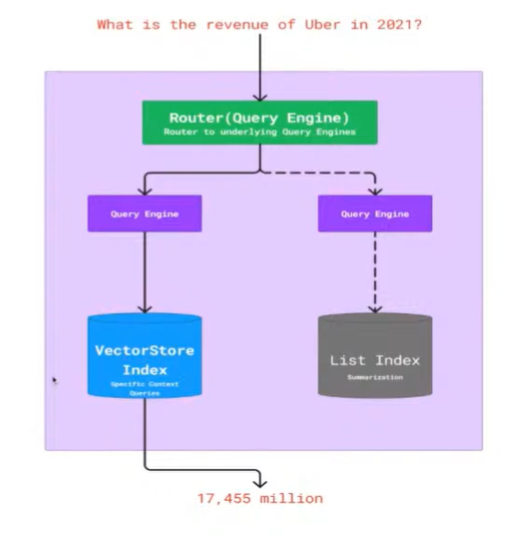
\includegraphics[width=0.5\linewidth,keepaspectratio]{llamaindex15}

{\tiny (Ref: LlamaIndex: A Central Interface between LLM’s + your external data)}
\end{center}
\end{frame}

%%%%%%%%%%%%%%%%%%%%%%%%%%%%%%%%%%%%%%%%%%%%%%%%%%%%%%%%%%%
\begin{frame}[fragile]\frametitle{Use Case: Document Comparison}

\begin{columns}
    \begin{column}[T]{0.45\linewidth}

		\begin{center}
		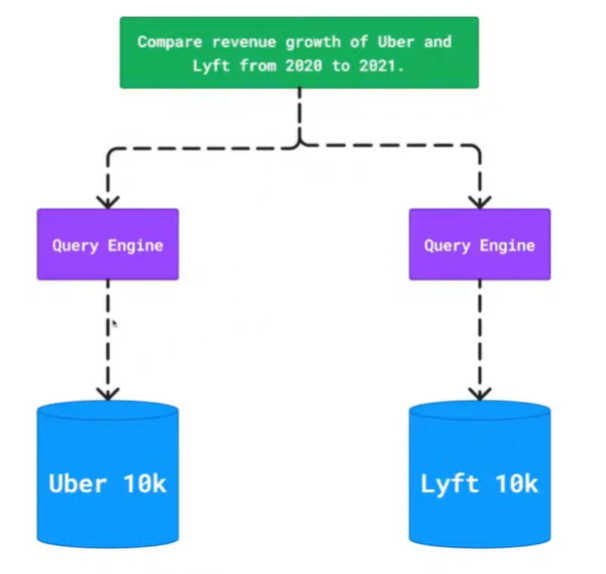
\includegraphics[width=\linewidth,keepaspectratio]{llamaindex16}

		{\tiny (Ref: Getting started with LlamaIndex - AI Planet)}
		\end{center}
		
    \end{column}
    \begin{column}[T]{0.45\linewidth}
		\begin{center}
		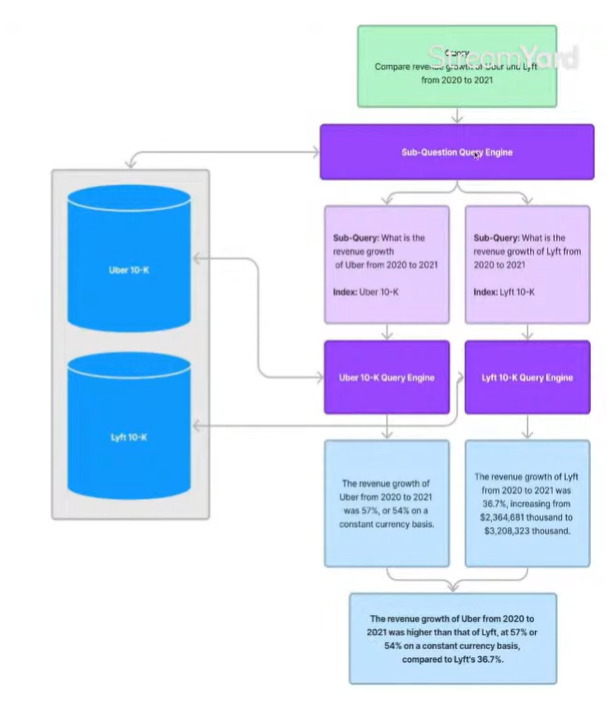
\includegraphics[width=\linewidth,keepaspectratio]{llamaindex17}

		{\tiny (Ref: Getting started with LlamaIndex - AI Planet)}
		\end{center}
    \end{column}
  \end{columns}
  
  


\end{frame}



%%%%%%%%%%%%%%%%%%%%%%%%%%%%%%%%%%%%%%%%%%%%%%%%%%%%%%%%%%%
\begin{frame}[fragile]\frametitle{Use Case: Text-to-SQL (Structured Data)}

\begin{center}
\includegraphics[width=\linewidth,keepaspectratio]{llm31}

{\tiny (Ref: LlamaIndex: A Central Interface between LLM’s + your external data)}
\end{center}
\end{frame}

%%%%%%%%%%%%%%%%%%%%%%%%%%%%%%%%%%%%%%%%%%%%%%%%%%%%%%%%%%%
\begin{frame}[fragile]\frametitle{Use Case: Synthesis over Heterogeneous Data}

Composing an index over other indexes (a list index over vector indexes). 
The query will be routed to both simple vector indexes! 


\begin{center}
\includegraphics[width=\linewidth,keepaspectratio]{llm32}

{\tiny (Ref: LlamaIndex: A Central Interface between LLM’s + your external data)}
\end{center}
\end{frame}

%%%%%%%%%%%%%%%%%%%%%%%%%%%%%%%%%%%%%%%%%%%%%%%%%%%%%%%%%%%
\begin{frame}[fragile]\frametitle{Composite Document: Text + Tables}


\begin{columns}
    \begin{column}[T]{0.4\linewidth}

		\begin{itemize}
		\item Recursive Retrieval expands exploration from directly relevant nodes to related retrievers/query engines
		\item Nodes representing table summaries, link to SQL or Pandas query engines for additional data
		\item If an IndexNode is fetched during a query, the associated query engine is queried
		\end{itemize}	
		
    \end{column}
    \begin{column}[T]{0.6\linewidth}
		\begin{center}
		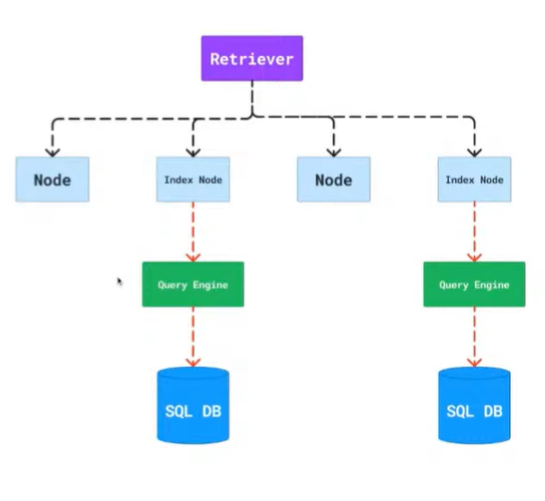
\includegraphics[width=\linewidth,keepaspectratio]{llamaindex18}

		{\tiny (Ref: Getting started with LlamaIndex - AI Planet)}
		\end{center}
    \end{column}
  \end{columns}
  


\end{frame}

%%%%%%%%%%%%%%%%%%%%%%%%%%%%%%%%%%%%%%%%%%%%%%%%%%%%%%%%%%%
\begin{frame}[fragile]\frametitle{Use Case: Compare/Contrast Queries}

https://github.com/jerryjliu/llama\_index/blob/main/examples/composable\_indices/city\_analysis/City\_Analysis-Decompose.ipynb

\begin{center}
\includegraphics[width=0.5\linewidth,keepaspectratio]{llm33}

{\tiny (Ref: LlamaIndex: A Central Interface between LLM’s + your external data)}
\end{center}
\end{frame}

%%%%%%%%%%%%%%%%%%%%%%%%%%%%%%%%%%%%%%%%%%%%%%%%%%%%%%%%%%%
\begin{frame}[fragile]\frametitle{Use Case: Multi-Step Queries}

\begin{itemize}
\item Break a complex query into multiple simpler ones! 
\item Chain-of-thought prompting over an existing data source.
\item https://github.com/jerryjliu/llama\_index/blob/main/
examples/vector\_indices/SimpleIndexDemo-multistep.ipynb
\end{itemize}	

\end{frame}


%%%%%%%%%%%%%%%%%%%%%%%%%%%%%%%%%%%%%%%%%%%%%%%%%%%%%%%%%%%
\begin{frame}[fragile]\frametitle{Use Case: Compare/Contrast Queries}


\begin{center}
\includegraphics[width=0.8\linewidth,keepaspectratio]{llm34}

{\tiny (Ref: LlamaIndex: A Central Interface between LLM’s + your external data)}
\end{center}
\end{frame}


%%%%%%%%%%%%%%%%%%%%%%%%%%%%%%%%%%%%%%%%%%%%%%%%%%%%%%%%%%%
\begin{frame}[fragile]\frametitle{Use Case: Exploiting Temporal Relationships}

\begin{columns}
    \begin{column}[T]{0.4\linewidth}
		\begin{itemize}
		\item Given a question, what if we would like to retrieve additional context in the past or the future?
		\item Example question: “What did the author do after his time at Y Combinator?” 
		\item Requires looking at context in the future! 
		\end{itemize}	
    \end{column}
    \begin{column}[T]{0.6\linewidth}
		\begin{center}
		\includegraphics[width=\linewidth,keepaspectratio]{llm35}

		{\tiny (Ref: LlamaIndex: A Central Interface between LLM’s + your external data)}
		\end{center}
    \end{column}
  \end{columns}
\end{frame}


%%%%%%%%%%%%%%%%%%%%%%%%%%%%%%%%%%%%%%%%%%%%%%%%%%%%%%%%%%%
\begin{frame}[fragile]\frametitle{Use Case: Recency Filtering / Outdated nodes}

\begin{columns}
    \begin{column}[T]{0.4\linewidth}
		\begin{itemize}
		\item Imagine you have three timestamped versions of the same data.
		\item If you ask a question over this data, you want to make sure it’s over the latest document.
		\end{itemize}	
    \end{column}
    \begin{column}[T]{0.6\linewidth}
		\begin{center}
		\includegraphics[width=0.6\linewidth,keepaspectratio]{llm36}

		{\tiny (Ref: LlamaIndex: A Central Interface between LLM’s + your external data)}
		\end{center}
    \end{column}
  \end{columns}
\end{frame}

%%%%%%%%%%%%%%%%%%%%%%%%%%%%%%%%%%%%%%%%%%%%%%%%%%%%%%%%%%%
\begin{frame}[fragile]\frametitle{Evaluation}

\begin{columns}
    \begin{column}[T]{0.4\linewidth}
		\begin{itemize}
		\item What is the need for evaluation?
		\item Question Generator.
		\item Evaluators.
		\end{itemize}	
    \end{column}
    \begin{column}[T]{0.6\linewidth}
		\begin{center}
		\includegraphics[width=0.6\linewidth,keepaspectratio]{llm39}

		{\tiny (Ref: LlamaIndex: A Central Interface between LLM’s + your external data)}
		\end{center}
    \end{column}
  \end{columns}
\end{frame}

%%%%%%%%%%%%%%%%%%%%%%%%%%%%%%%%%%%%%%%%%%%%%%%%%%%%%%%%%%%
\begin{frame}[fragile]\frametitle{Response Evaluator}

\begin{columns}
    \begin{column}[T]{0.4\linewidth}
Takes in response source information and output response to evaluate the correctness of the response.

    \end{column}
    \begin{column}[T]{0.6\linewidth}
		\begin{center}
		\includegraphics[width=0.6\linewidth,keepaspectratio]{llm40}

		{\tiny (Ref: LlamaIndex: A Central Interface between LLM’s + your external data)}
		\end{center}
    \end{column}
  \end{columns}
\end{frame}

%%%%%%%%%%%%%%%%%%%%%%%%%%%%%%%%%%%%%%%%%%%%%%%%%%%%%%%%%%%
\begin{frame}[fragile]\frametitle{Query Response Evaluator}

\begin{columns}
    \begin{column}[T]{0.4\linewidth}
Takes in Query, response source information and output response to evaluate the correctness of the response.

    \end{column}
    \begin{column}[T]{0.6\linewidth}
		\begin{center}
		\includegraphics[width=0.6\linewidth,keepaspectratio]{llm41}

		{\tiny (Ref: LlamaIndex: A Central Interface between LLM’s + your external data)}
		\end{center}
    \end{column}
  \end{columns}
\end{frame}


%%%%%%%%%%%%%%%%%%%%%%%%%%%%%%%%%%%%%%%%%%%%%%%%%%%%%%%%%%%
\begin{frame}[fragile]\frametitle{Source Context Evaluation}

\begin{columns}
    \begin{column}[T]{0.4\linewidth}
Takes in Query, each source information and output response to evaluate the correctness of the response.

    \end{column}
    \begin{column}[T]{0.6\linewidth}
		\begin{center}
		\includegraphics[width=0.6\linewidth,keepaspectratio]{llm42}

		{\tiny (Ref: LlamaIndex: A Central Interface between LLM’s + your external data)}
		\end{center}
    \end{column}
  \end{columns}
\end{frame}



%%%%%%%%%%%%%%%%%%%%%%%%%%%%%%%%%%%%%%%%%%%%%%%%%%%%%%%%%%%
\begin{frame}[fragile]\frametitle{Integration into Downstream Apps}

\begin{columns}
    \begin{column}[T]{0.4\linewidth}
		\begin{itemize}
		\item Build a Streamlit app! 
		\item https://huggingface.co/spaces/llamaindex/llama\_index\_sql\_sandbox
		\end{itemize}	
    \end{column}
    \begin{column}[T]{0.6\linewidth}
		\begin{center}
		\includegraphics[width=\linewidth,keepaspectratio]{llm37}

		{\tiny (Ref: LlamaIndex: A Central Interface between LLM’s + your external data)}
		\end{center}
    \end{column}
  \end{columns}
\end{frame}

%%%%%%%%%%%%%%%%%%%%%%%%%%%%%%%%%%%%%%%%%%%%%%%%%%%%%%%%%%%
\begin{frame}[fragile]\frametitle{Integration into Downstream Apps}

\begin{columns}
    \begin{column}[T]{0.4\linewidth}
		\begin{itemize}
		\item Building a unified query interface
		\item https://colab.research.google.com/drive/
		1KH8XtRiO5spa8CT7UrXN54IWdZk3DDxl?usp=sharing
		\end{itemize}	
    \end{column}
    \begin{column}[T]{0.6\linewidth}
		\begin{center}
		\includegraphics[width=0.6\linewidth,keepaspectratio]{llm38}

		{\tiny (Ref: LlamaIndex: A Central Interface between LLM’s + your external data)}
		\end{center}
    \end{column}
  \end{columns}
\end{frame}
